\chapter{Luminometer Calibration}
\label{ch3}

\section{Van Der Meer Method}

The Van Der Meer (vdM) scan let us obtain the value of $\sigma_{visible}$ using different luminometers. For this case the detector of interest is the pixel detector with which are going to obtain a calibration of the luminosity using the vdM scan in combination with the PCC method. The scan consist on separating particle the beams from each other between the X and Y axis by $\Delta X$ and $\Delta Y$ values moving them and recording values of luminosity independently, when the scan on X and scan on Y are imposed over each other we said that they're on head on giving the maximum value of luminosity. Usually a single gaussian fit is used to obtain beam overlap widths also denoted as $\Sigma_{x}$ and $\Sigma_{y}$, other fit models may be used like the doble gaussian depending on the quality of the fit \cite{Vdm}

\begin{figure}[h]
    \centering
    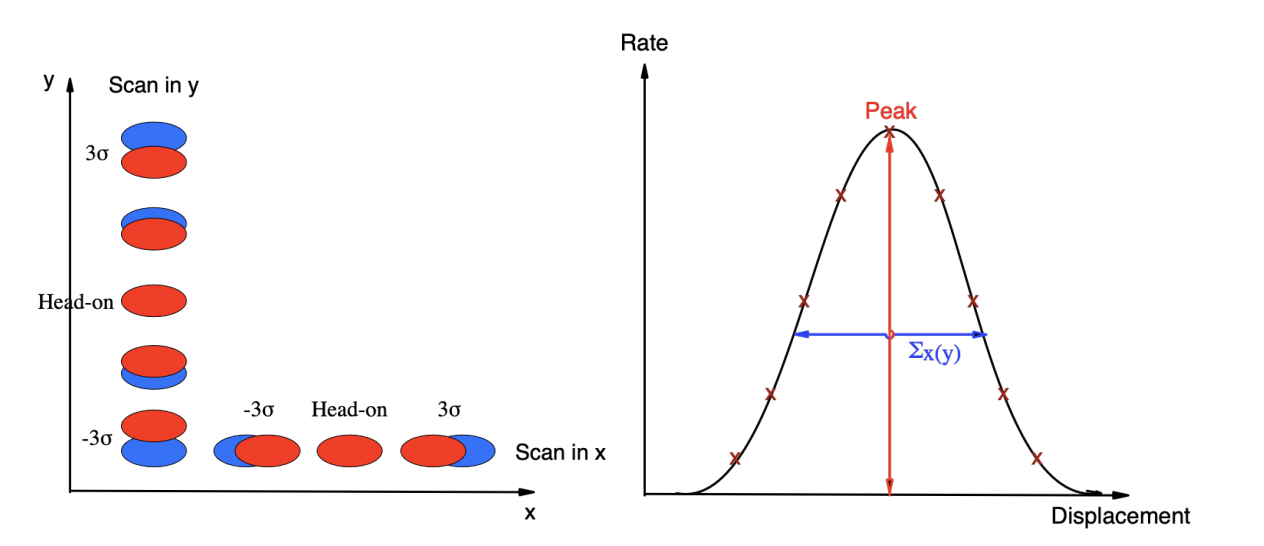
\includegraphics[width=1\textwidth]{vdm1.png}
    \caption{The vdm scan on the left showing the beams for X and Y. On the right a curve of the different values of rate for the beams displacement, the peak occurs during the head on part.}
    \label{fig:vdm1}
\end{figure}


For obtaining the importnat parameters on the vdm scan we return to the equation (1.2) and apply it to and individual bunch crossing, the values of N1 and N2 being the number of protons colliding can be obtained since is a known quantity from the experiment, the frequency f is also a known quantity, the frequency of the LHC which is 11,245 kHz but the proton densities $\rho_{1}$ and $\rho{2}$ are more difficult to obtain, this is were the vdM scan help us to measure integral over the bunch proton densities. The luminosity integral evaluated with the beams separated by a distance $\Delta_{x}$ and $\Delta_{y}$ can take the form of: 

\begin{equation}
 L(\Delta x, \Delta Y) = N_{1} N_{2} f  \int \int \rho_{1}(x,y)\rho_{2}(x+\Delta x, y+\Delta y) dxdy 
\end{equation}

Because of the scan method is it assumed that the two bunches of proton densities are factorizable since they act independently between each other so we can turn the right part of (3.1) into two integrals:

 \begin{equation}
N_{1} N_{2} f  \int \int \rho_{1}(x,y)\rho_{2}(x+\Delta x, y+\Delta y) dxdy   = N_{1} N_{2} f (\int \rho_{1}(x)\rho_{2}(x + \Delta x) dx) (\int rho_{1}(y) \rho_{2}(y + \Delta y) dy)
\end{equation}

Integrating both sides on $\Delta y$ and using in combination with (3.1) while we fix $\Delta x_{0}$ = 0 and $\Delta y_{0}$ = 0 as the head on point,  we obtain:
 
 \begin{equation}
N_{1} N_{2} f \int \rho_{1}(x) \rho_{2}(x + \Delta x_{0}) dx = \int L (\Delta x_{0}, d\Delta y) d(\Delta y)
\end{equation}

A similar result is obtained when we integrate both sides for $\Delta x$ using this and combining equation (3.1), (3.2) and (3.3) we can obtain that 

\begin{equation}
N_{1} N_{2} f \int \rho_{1}(x) \rho_{2}(x + \Delta x_{0}) dx = \frac{L (\Delta X_{0}, Delta y_{0})}{\int L(\Delta x_{0}, \Delta y) d(\Delta y)}
\end{equation}

Similarly to the previous step we can obtain the value of the other factor of (3.2) with an analogous process. The integrals resulting on the right side can be evaluated by evaluated by obtaining the rate in function of the beam-beam separation which are $\Delta x$ and $\Delta y$  this because the luminosity has a linear relationship with the rate. The Luminosity can be expresed on terms of the rate during the head on points using the following:

\begin{equation}
L(\Delta x, \Delta y) = N_{1} N_{2} f \frac{2R(\Delta x_{0}, \Delta y_{0}}{\int L(\Delta x_{0}, \Delta y) d(\Delta y) \int L(\Delta x, \Delta y_{0}) d(\Delta x)}
\end{equation}

Here the luminosity is replaced by the rate R, it is convenient to write this integral in terms of the convoluted beam widths which are denoted by $\Sigma_{x}$ and $\Sigma_{Y}$, this convoluted widths are defined by: 

\begin{equation}
\Sigma_{x} = \frac{1}{2 \pi} \frac{\int R(\Delta x, \Delta y_{0} d(\Delta x) )}{R(\Delta x_{0}, \Delta y_{0})}
\end{equation}

For $\Sigma_{y}$ the result is analogous. With (3.6) we can write (3.5) in a different manner:

\begin{equation}
L(\Delta x, \Delta y) = \frac{N_{1}N_{2}f}{2 \pi \Sigma_{x} \Sigma_{y}}
\end{equation}  

This in combination with (1.4) make us possible to obtain the following expression for the visible cross section

\begin{equation}
\sigma_{vis} = \frac{2 \pi \Sigma_{x} Sigma_{y} R(\Delta x_{0} \Delta y_{0})}{N_{1} N_{2}f}
\end{equation}

This makes possible obtain $\sigma_{vis}$ only by experiment since all of the right values can be obtained via the experiment, the maximum rate R($\Delta x_{0}$, $\Delta y_{0}$) is obtained at the maximum PCC obtained during the vdm scan, this means during the head-on process, while the $\Sigma_{x}$ and $\Sigma_{y}$ are obtained with the information of the fit model. 

This calculations are done on several Bunch Cross Identifier which so you obtain several values of $\simga_{vis}$ and then they are weight averaged according to the uncertainties in order to obtain $\sigma_{vis}$ for the scan. 

\section{Datasets}

The data on the CMS is a complex set of inter-dependent workflows made in a way that assure the full physics exploitation of the CMS detector potential and the collisions delivered by the LHC, this data provides analyses with reconstructed collision events from the experiment and are designed to use the CMS computing resources efficiently. This stream of events is organized into datasets according to the results of the High Level Trigger (HLT) which defines primary datasets since they are defined by the paths of the HLT. The design of the primary datasets is centered around candidates for particles that are reconstructed on the final state by the hLT and follows the principle of grouping together events with similar physics content.    \cite{datasets1}

The datasets used for the obtention of the $\sigma_{visible}$ for 2024 were the ones from the Fill 9639 which is divided in 3 blocks, a fill is a process that generates beams for the LHC this tipycally involves particles around the number of $10^{14}$ that are grouped in bunches that form the proton beam. This is what we use the bcid number to identify this bunches, there are a total of 3564 bunches that are empty or filled depending on the fill all of this part of the LHC bunch train. For this fill in the calibration the bcids of relevance were a total of 12 which are identified by the numbers: 303, 324, 345, 506, 527, 822, 1081, 1102, 1397, 2000, 2965, 3123. This fill started on may 16 at 13:39 and ended at may 17 at 23:50.

In the case for our datasets each bcid is processed by the CMS collaboration to enable cluster reconstruction resulting in the ALCARECO datasets that contain a module collection and their number of cluster per event in CMSWW format. This samples are processed using the CMSWW software to extract the clusters per module to obtain the dataset in the ROOT format. ROOT is a software framework born at CERN It is open source and used for high energy physics to analyze data while providing packages for storage, processing and visualization while minimizes the computing resources needed. 

The root format saves the data in form of TTrees which behaves like an array of data structure and storage data. This tree consist on branches and leaves, a branch is a list of independent columns that can contain values of any fundamental type and are represented by TBranch. While the leaves represented by TLeaf give access to actual data in difference to the TBranch which represent a structure. After the datasets are processed, the rates of the Pixel detector were stored each 1.32 seconds periods called NB4 this to make an average of clusters and the number of events that fall into that time span. 

This dataset were processed (...) getting a lot of root files for each of the different zero bias streams there were a total of 32 zero bias streams. The data then was processed again to obtain a hd5file a format that can supports n-dimensional datasets and facilitates the reading of the datasets, this hd5 files contained relevant information about the root files like the average rate per NB4, this was made for each of the files for almost all of the available streams excluding two of them that were not ready by the moment (the ones that were identified by ZB21 and ZB28) after one stream got all of his files processed into an hd5 file they were converged into a single file containing relevant information for all the stream, once all of the files in all of the data streams were processed into hd5 files a single hd5file was made containing all of the information about the streams also a single csv file was made containing only the average rate file per NB4 for each of the bcids.  
 
\section{Scans}

During the duration of the fill and for the calibration a few scans of interest were realized the first of them being the vdm scans which was explained in the first section of the chapter, also the BI scans, there were a total of five vdm scans during and two BI scans in the following table we see the time were this scans started and the time w    \\



Also we got the super separation scans which consist on making a complete separation on the colliding beams so the rate would be zero, there were five of each super separations each of them with a duration of 300 seconds in the table we have information about the beggining and end of each super separation (SS) period. 

\begin{table} [H]
\begin{center}
\caption{Super Separation Period time}
\begin{tabular}{|c c c|} 
 \hline
 Scan & Time Start & Time End  \\ [0.5ex] 
 \hline\hline
 SS1 & 1715883182 & 1715883481  \\ 
 \hline
 SS2 & 1715902185 & 1715902484  \\
 \hline
 SS3 & 1715919164 & 1715919463 \\
 \hline
 SS6 & 1715943045 & 1715943343  \\
 \hline
 SS5 & 1715987303 & 1715987602  \\ [1.0ex]
 \hline
\end{tabular}
\end{center}
\end{table}

In the following image we show a histogram of the average rate vs time during the super separation period number 2: 

\begin{figure}[h]
    \centering
    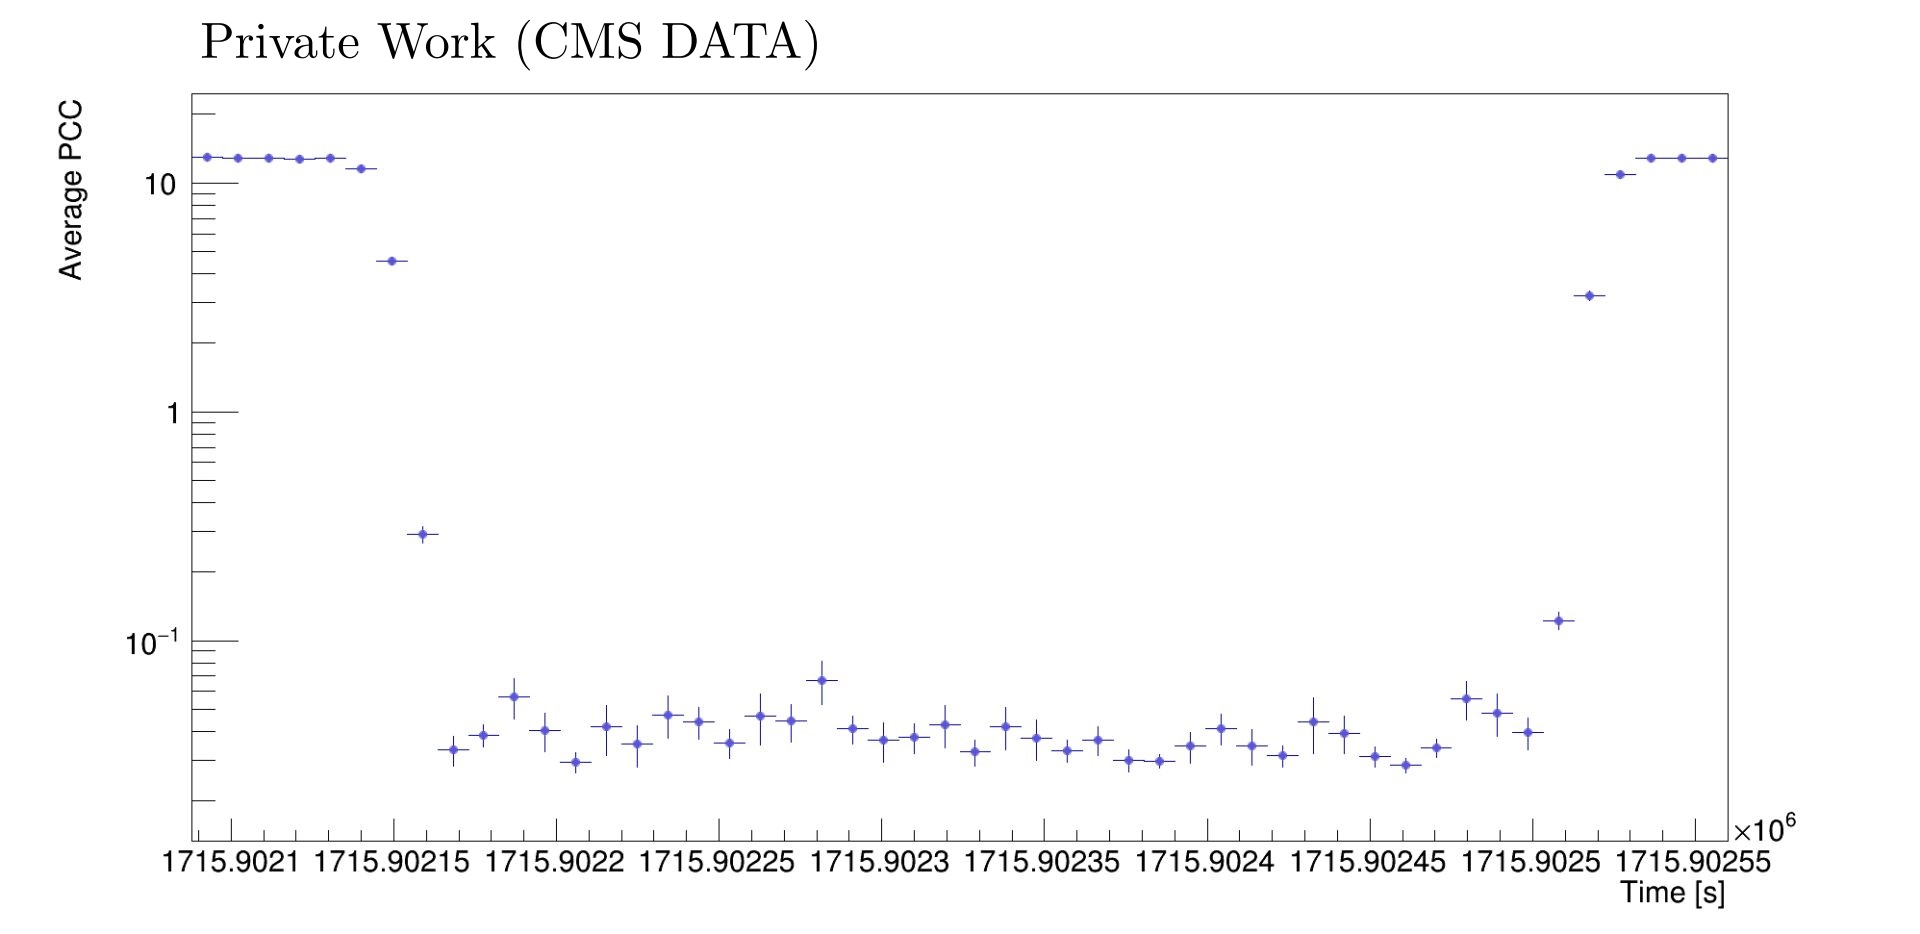
\includegraphics[width=1\textwidth]{SS1.jpeg}
    \caption{Histogram of rates during the second super separation scan}
    \label{fig:SS1}
\end{figure}

In the image we can see that the average rate suddenly drops, this is the beggining of the second super separation scan for the bcid 506 where the avarage rate drop but is non zero, then the rate goes up again meaning the end to the super separation scan.  

\section{Background Estimation}

The background estimation is obtained during the super separation (SS) process, since the SS scan separates the beams so they shouldn't be colliding the expected value on the rate is expected to be a rate associated with the background, this is then estimated by checking each of the SS scans on the time window referred on the table (3.1), the mean value during this period is assumed to be the mean value of the SS period, in the following table we see the mean PCC value for each period.  

\begin{table} [H]
\begin{center}
\caption{Different Scans}
\begin{tabular}{|c c c|} 
 \hline
 Scan & Mean & std  \\ [0.5ex] 
 \hline\hline
 SS1 &  & 1715883481  \\ 
 \hline
 SS2 &  & 1715902484  \\
 \hline
 SS3 &  & 1715919463 \\
 \hline
 SS6 &  & 1715943343  \\
 \hline
 SS5 &  & 1715987602  \\ [1.0ex]
 \hline
\end{tabular}
\end{center}
\end{table}

This is the mean value of each super separation off al the bcids a total of 60 mean values were obtained 


\section{Corrections}

\section{Fit model} 

There are different fit models at the time to do the vdm calibration, the most common one is Single Gaussian but also other models like the Double Gaussian, QG, Poly2g or Poly 4G. Each of these models have different parameters and restrictions making some of them better than other on the fit quality. 


\section{Beam Parameters}



